\documentclass{homework}
\usepackage[utf8]{inputenc}
\usepackage{amsmath}
\usepackage{amssymb}
\usepackage{braket}
\usepackage{graphicx}
\graphicspath{{./graphs/}} %location of images
\usepackage{xspace,color} % for R images & code
\usepackage{url}
\usepackage{listings}
\usepackage{subcaption}


\lstset{commentstyle=\color{red},keywordstyle=\color{black},
showstringspaces=false}
\lstnewenvironment{rc}[1][]{\lstset{language=R}}{}
\newcommand{\ri}[1]{\lstinline{#1}}  %% Short for 'R inline'

\lstset{language=R}             % Set R to default language

\newcommand{\hwname}{Shara Duong, Charles Colgan, Josh Borders}
\newcommand{\hwnum}{1}

\newcommand{\hwtype}{Homework}
\newcommand{\hwclass}{MATH 6350}

\begin{document}

\maketitle

**MEMBER CONTRIBUTIONS**

%Question 1
\question
\begin{rc}
           Cyl   Displ        HP    Weight     Accel
Mean   5.471939 194.412 104.46939 2977.5842 15.541327
StdDev 1.705783 104.644  38.49116  849.4026  2.758864
\end{rc}
This table displays the respective means and standard deviations of each feature in the Auto data set (n=392): number of Cylinders, Displacement (cubic in), Horsepower, Weight (lbs), and Acceleration (seconds required to accelerate from 0mph to 60mph). For example, the average car in the data set has a horsepower of 104.47, with a standard deviation of 38.49 horsepower.

%Question 2
\question
Below are the histograms for all five features and the response variable, mpg, with a normal distribution pdf curve overlayed. The variables acceleration and miles per gallon closely follow a normal distribution, while weight, horsepower, and displacement are left skew. Since cylinder is a categorical variable, it is not expected to be normally distributed.

\begin{figure}[h]
    \centering
    \begin{subfigure}[b]{0.3\textwidth}
        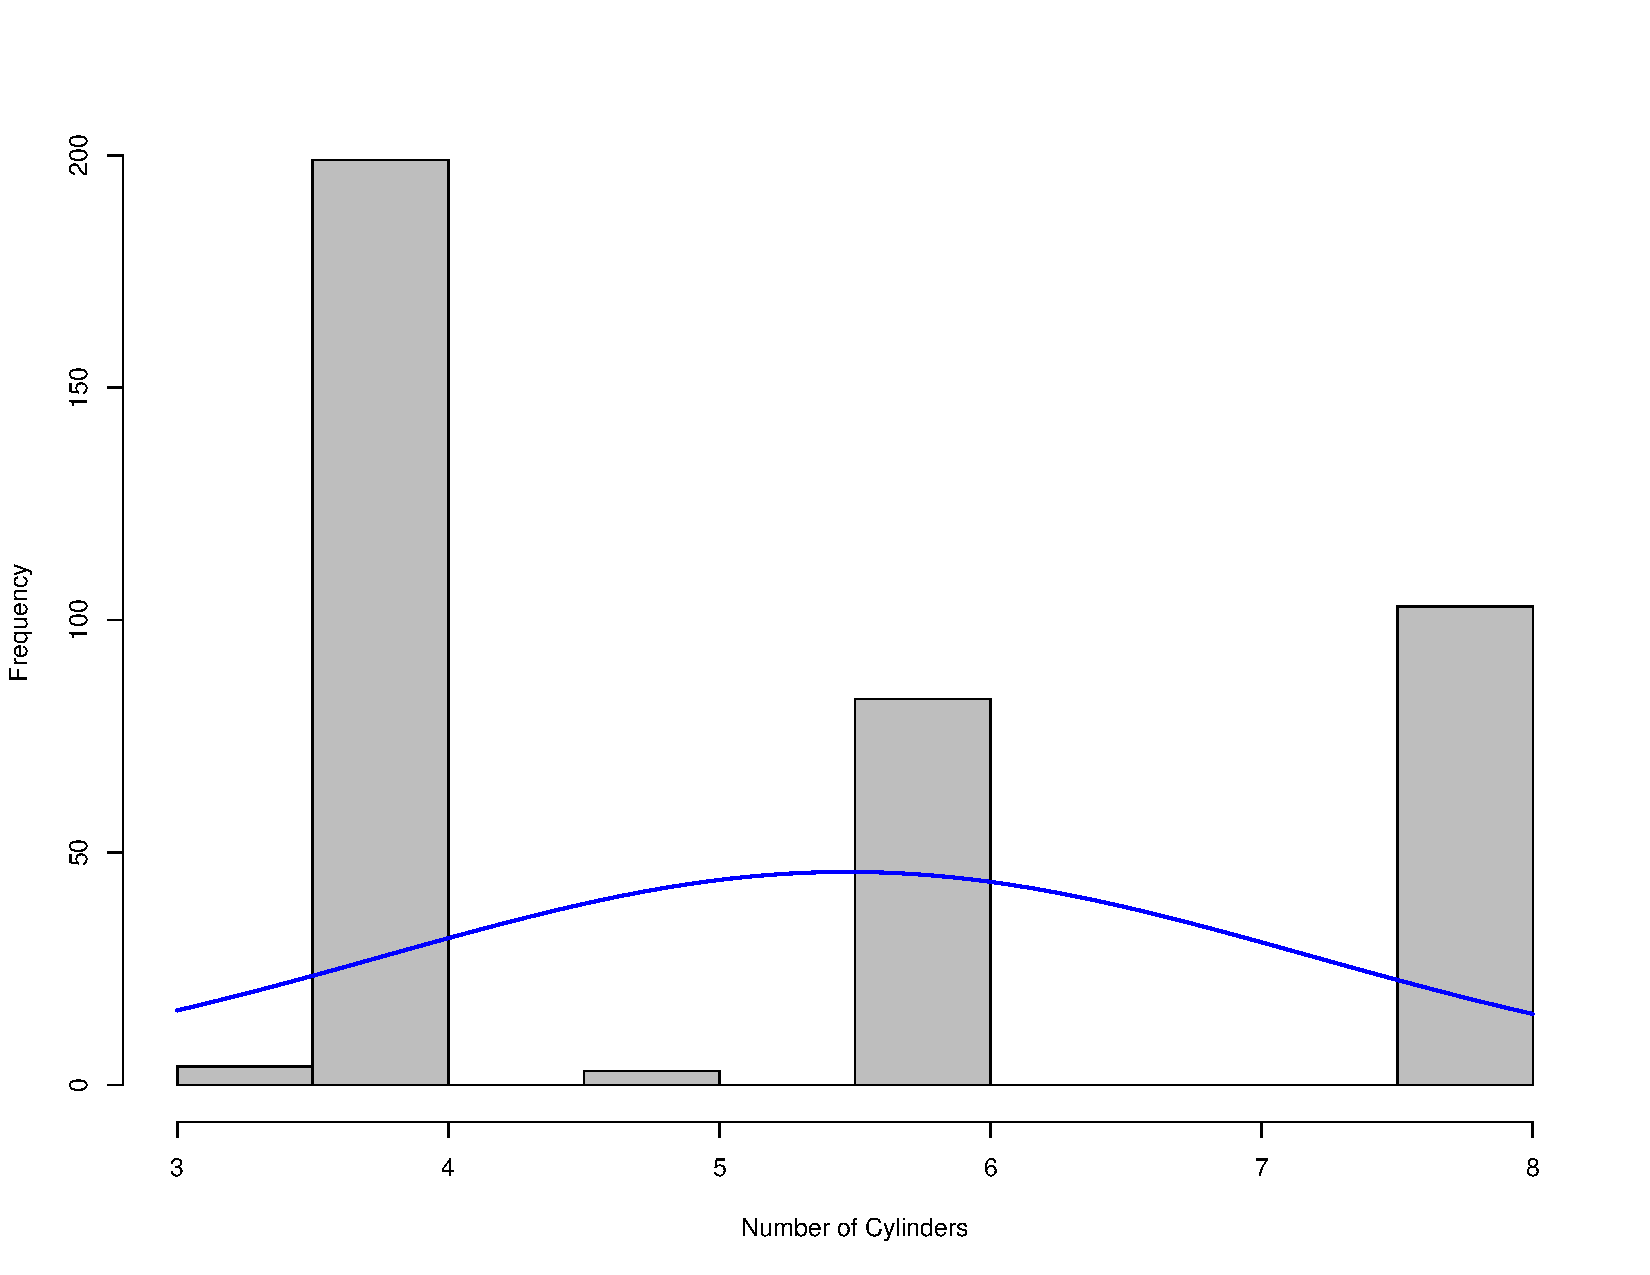
\includegraphics[width=\textwidth]{graphs/histCyl.pdf}
        \caption{cylinder}
        \label{fig:cylinder}
    \end{subfigure}
    \begin{subfigure}[b]{0.3\textwidth}
        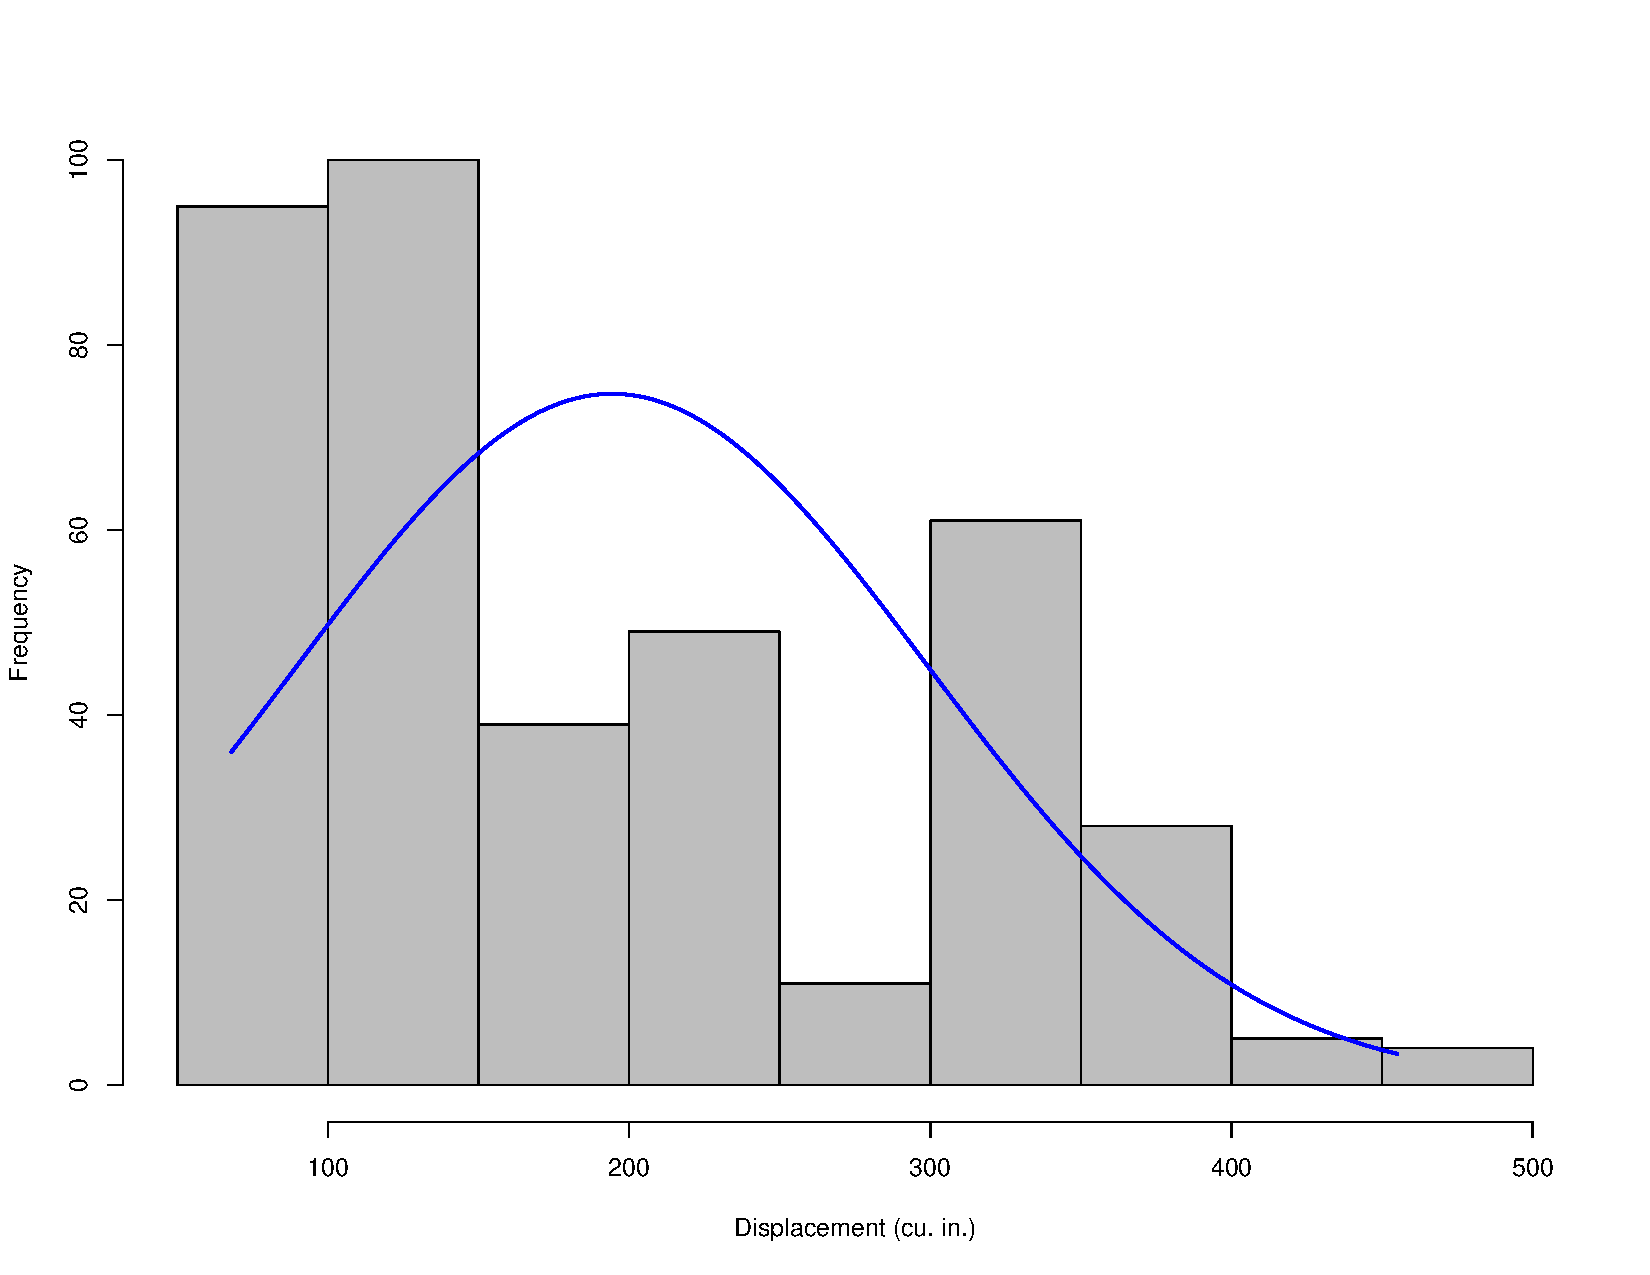
\includegraphics[width=\textwidth]{graphs/histDis.pdf}
        \caption{displacement}
        \label{fig:displacement}
    \end{subfigure}
    \begin{subfigure}[b]{0.3\textwidth}
        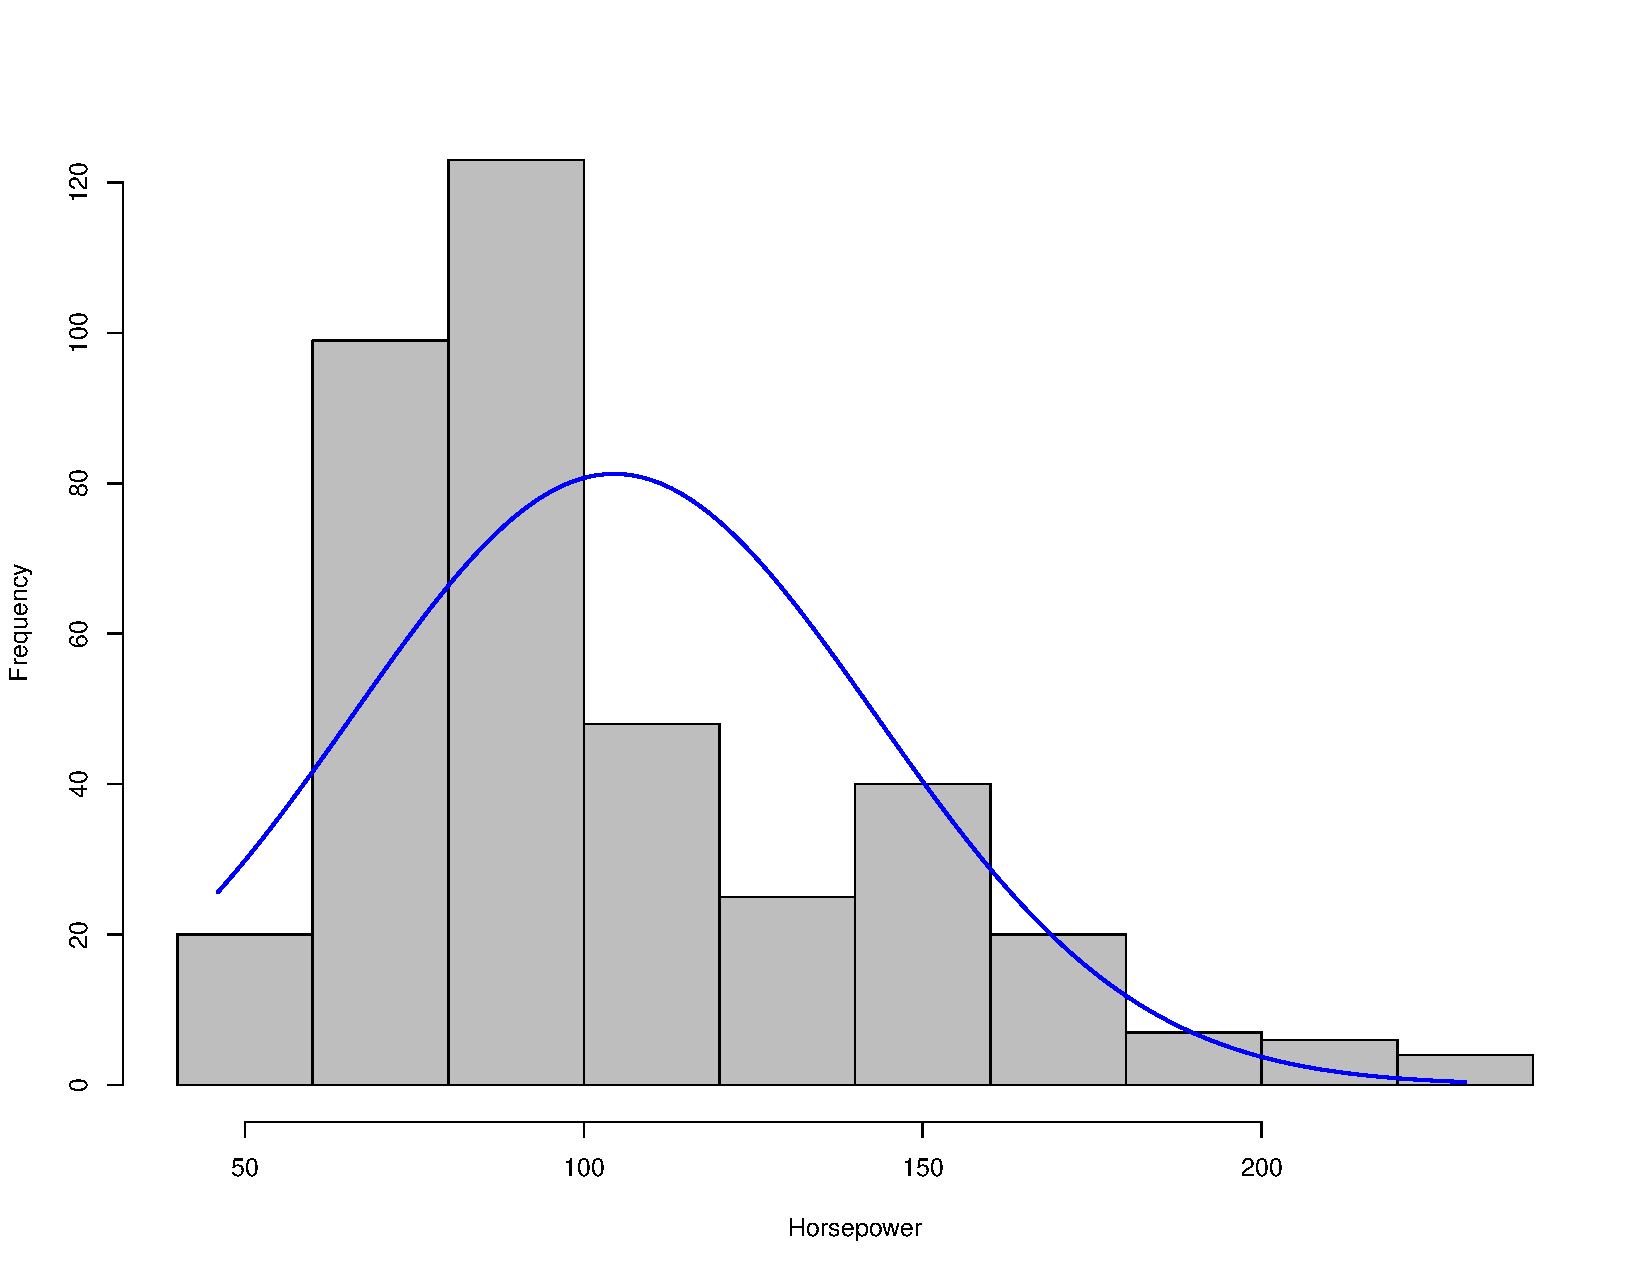
\includegraphics[width=\textwidth]{graphs/histHP.pdf}
        \caption{horsepower}
        \label{fig:HP}
    \end{subfigure}
    \begin{subfigure}[b]{0.3\textwidth}
        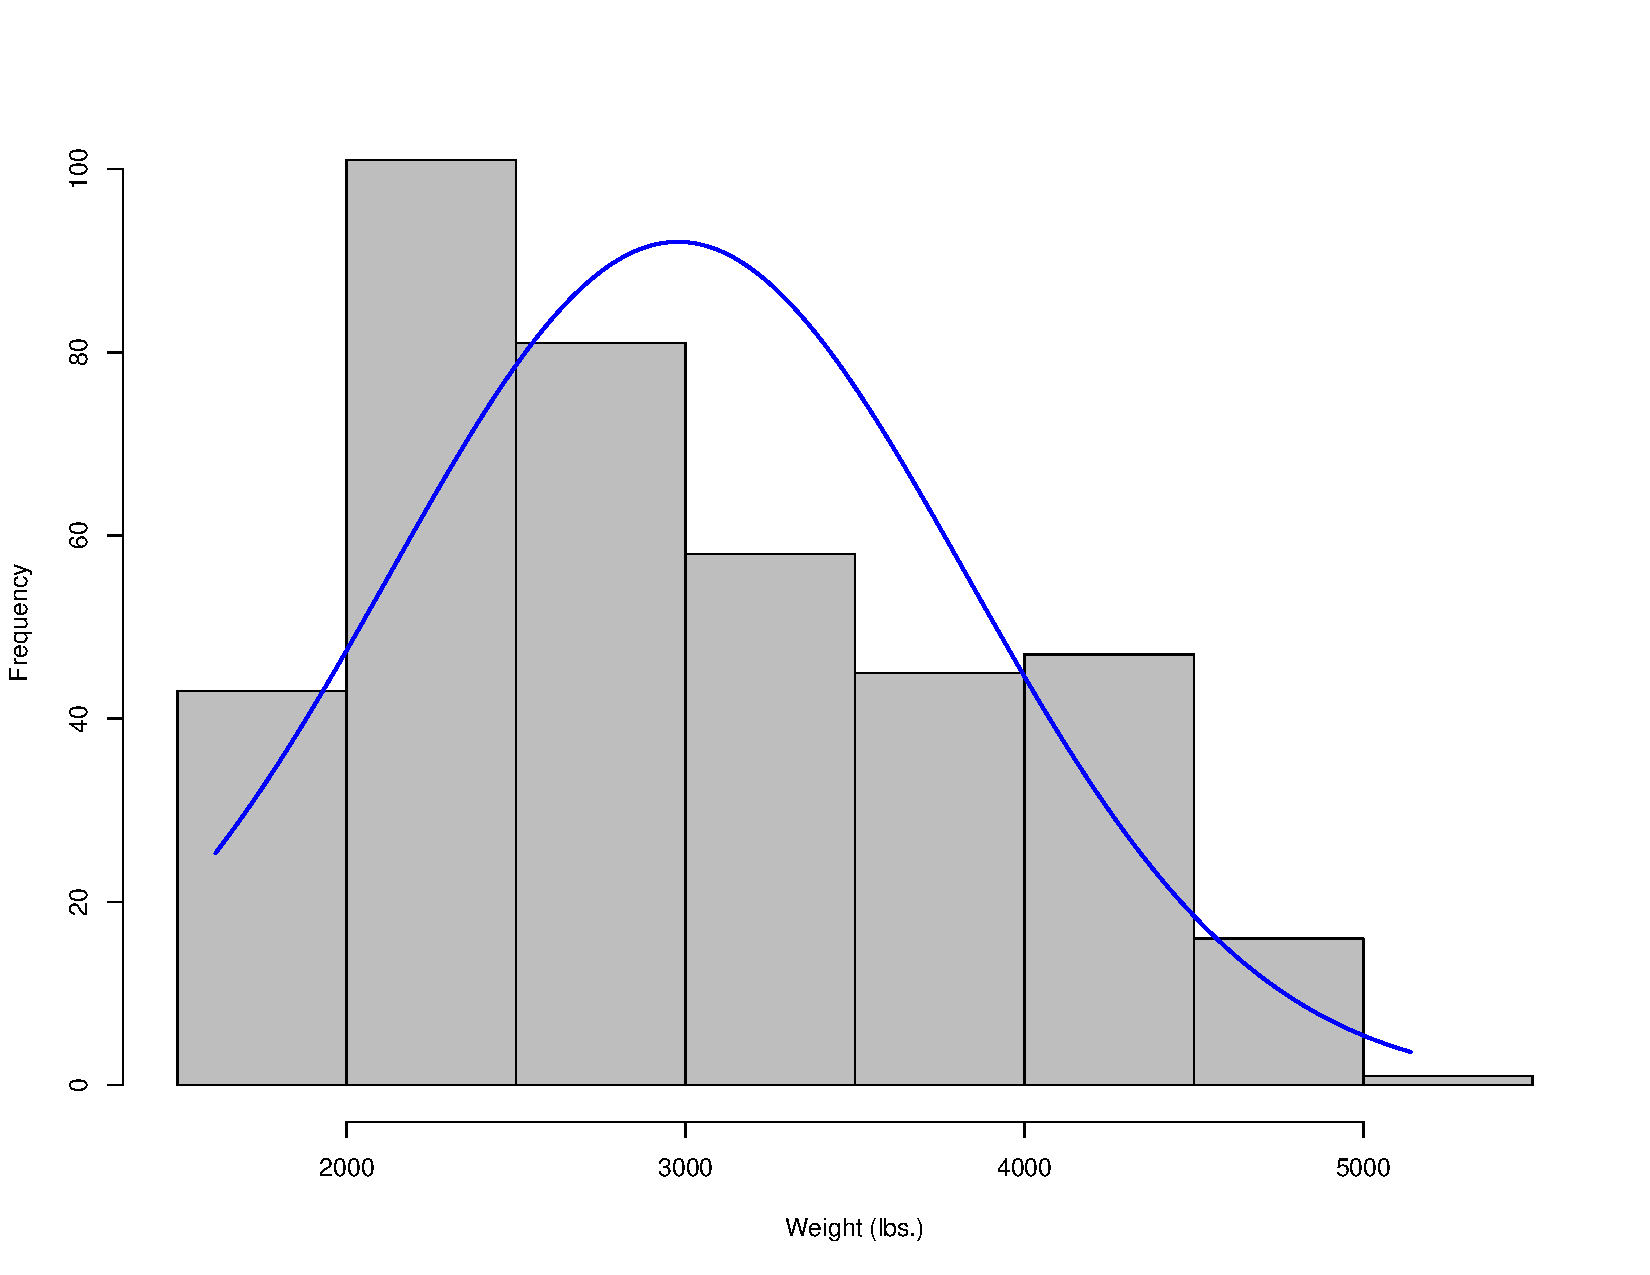
\includegraphics[width=\textwidth]{graphs/histWei.pdf}
        \caption{weight}
        \label{fig:HP}
    \end{subfigure}
    \begin{subfigure}[b]{0.3\textwidth}
        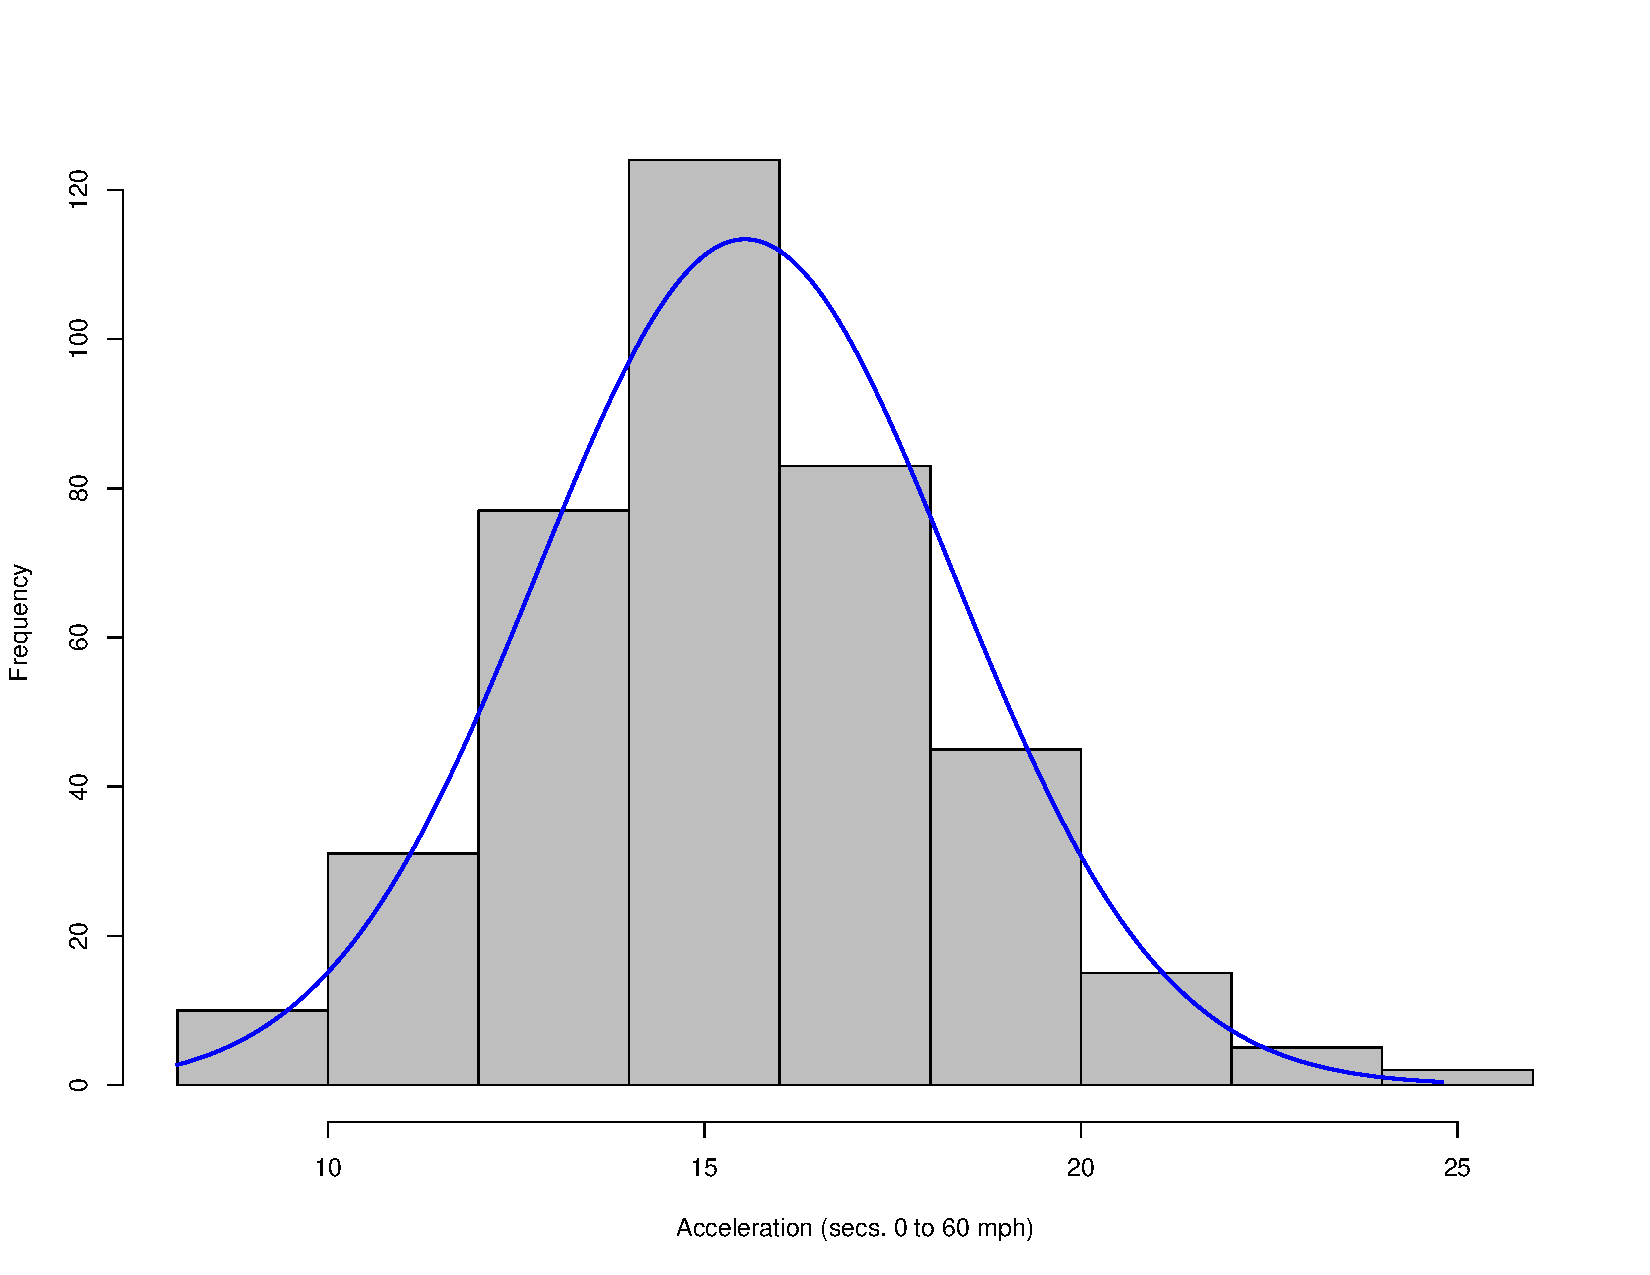
\includegraphics[width=\textwidth]{graphs/histAcc.pdf}
        \caption{acceleration}
        \label{fig:HP}
    \end{subfigure}
    \begin{subfigure}[b]{0.3\textwidth}
        \includegraphics[width=\textwidth]{graphs/histmpg.pdf}
        \caption{miles per gallon}
        \label{fig:HP}
    \end{subfigure}
    \caption{Histograms of Features with Normal PDF Overlay}\label{fig:features}
\end{figure}

%Question 3
\question
\begin{figure}
\centering
    \begin{subfigure}[b]{0.3\textwidth}
        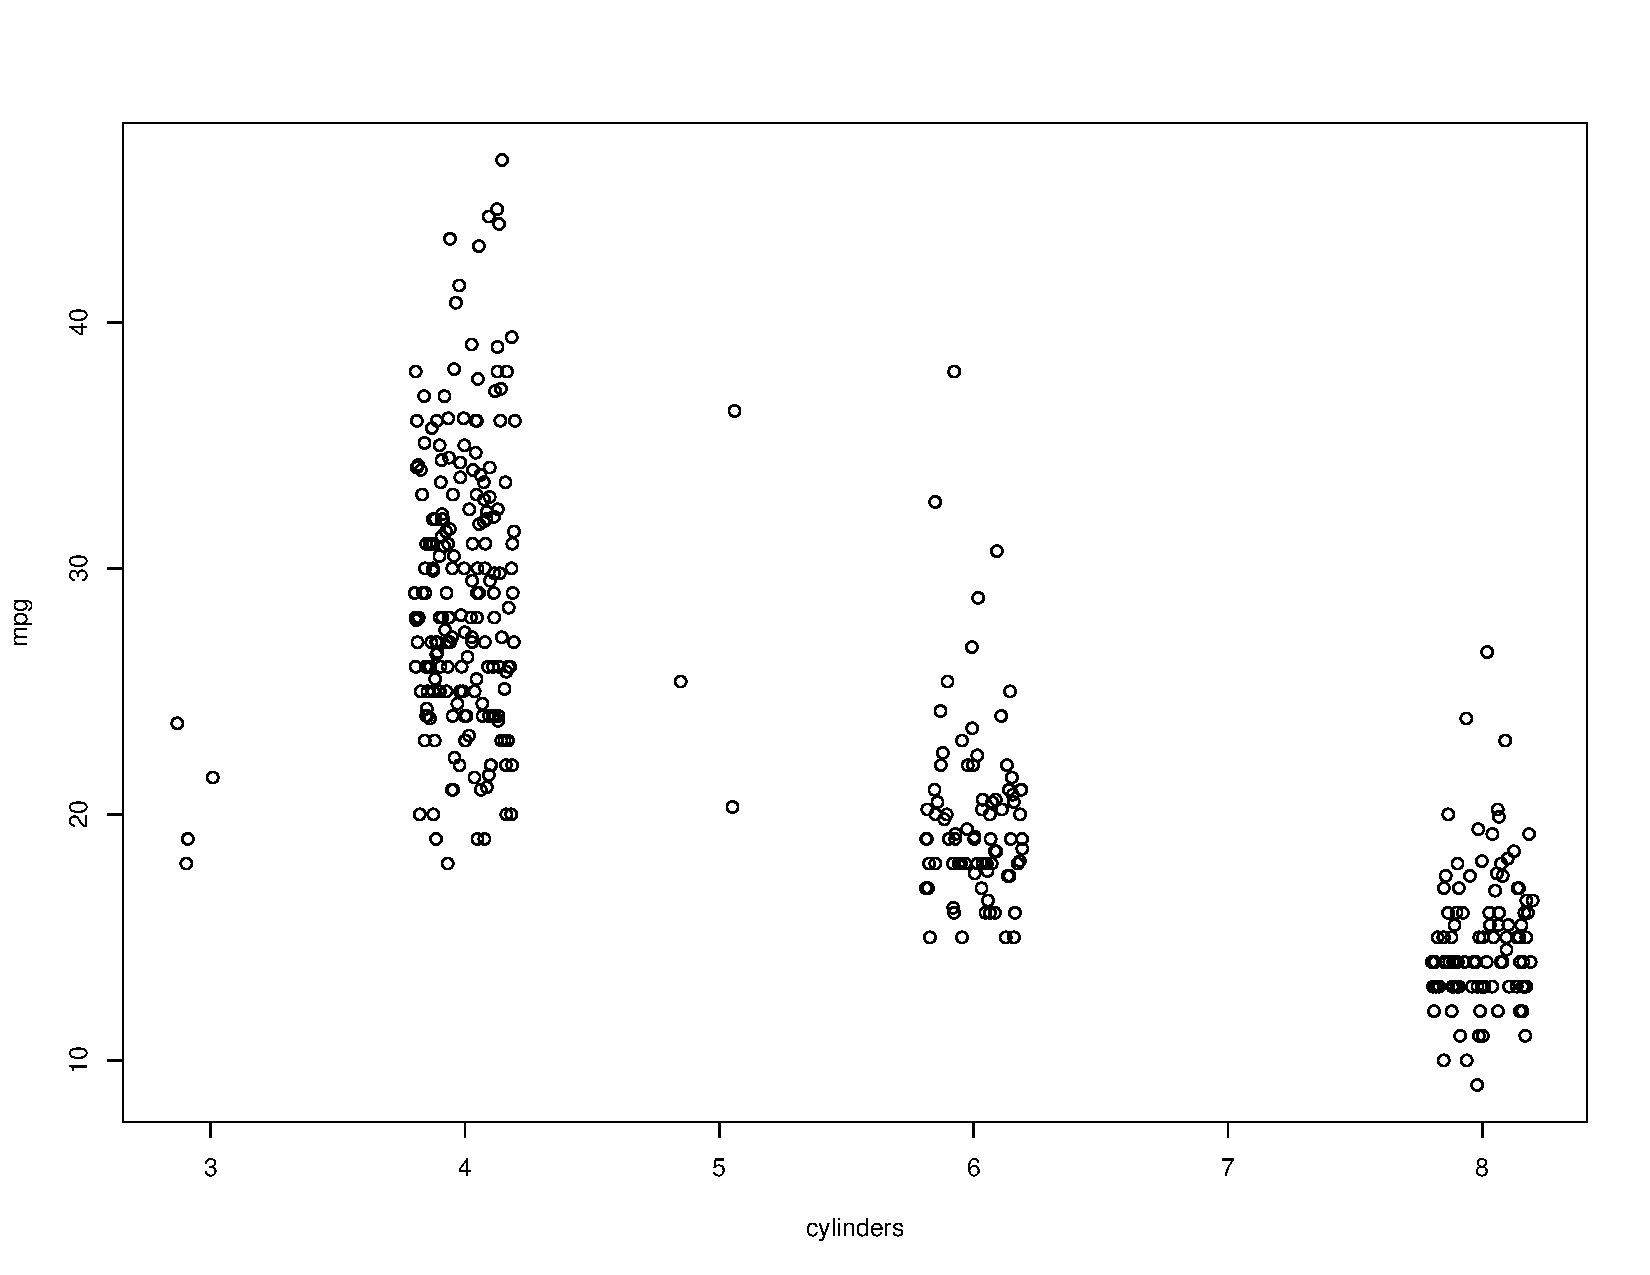
\includegraphics[width=\textwidth]{graphs/scatterCyl.pdf}
        \caption{(cylinders, mpg)}
        \label{fig:cylinder}
    \end{subfigure}
    \begin{subfigure}[b]{0.3\textwidth}
        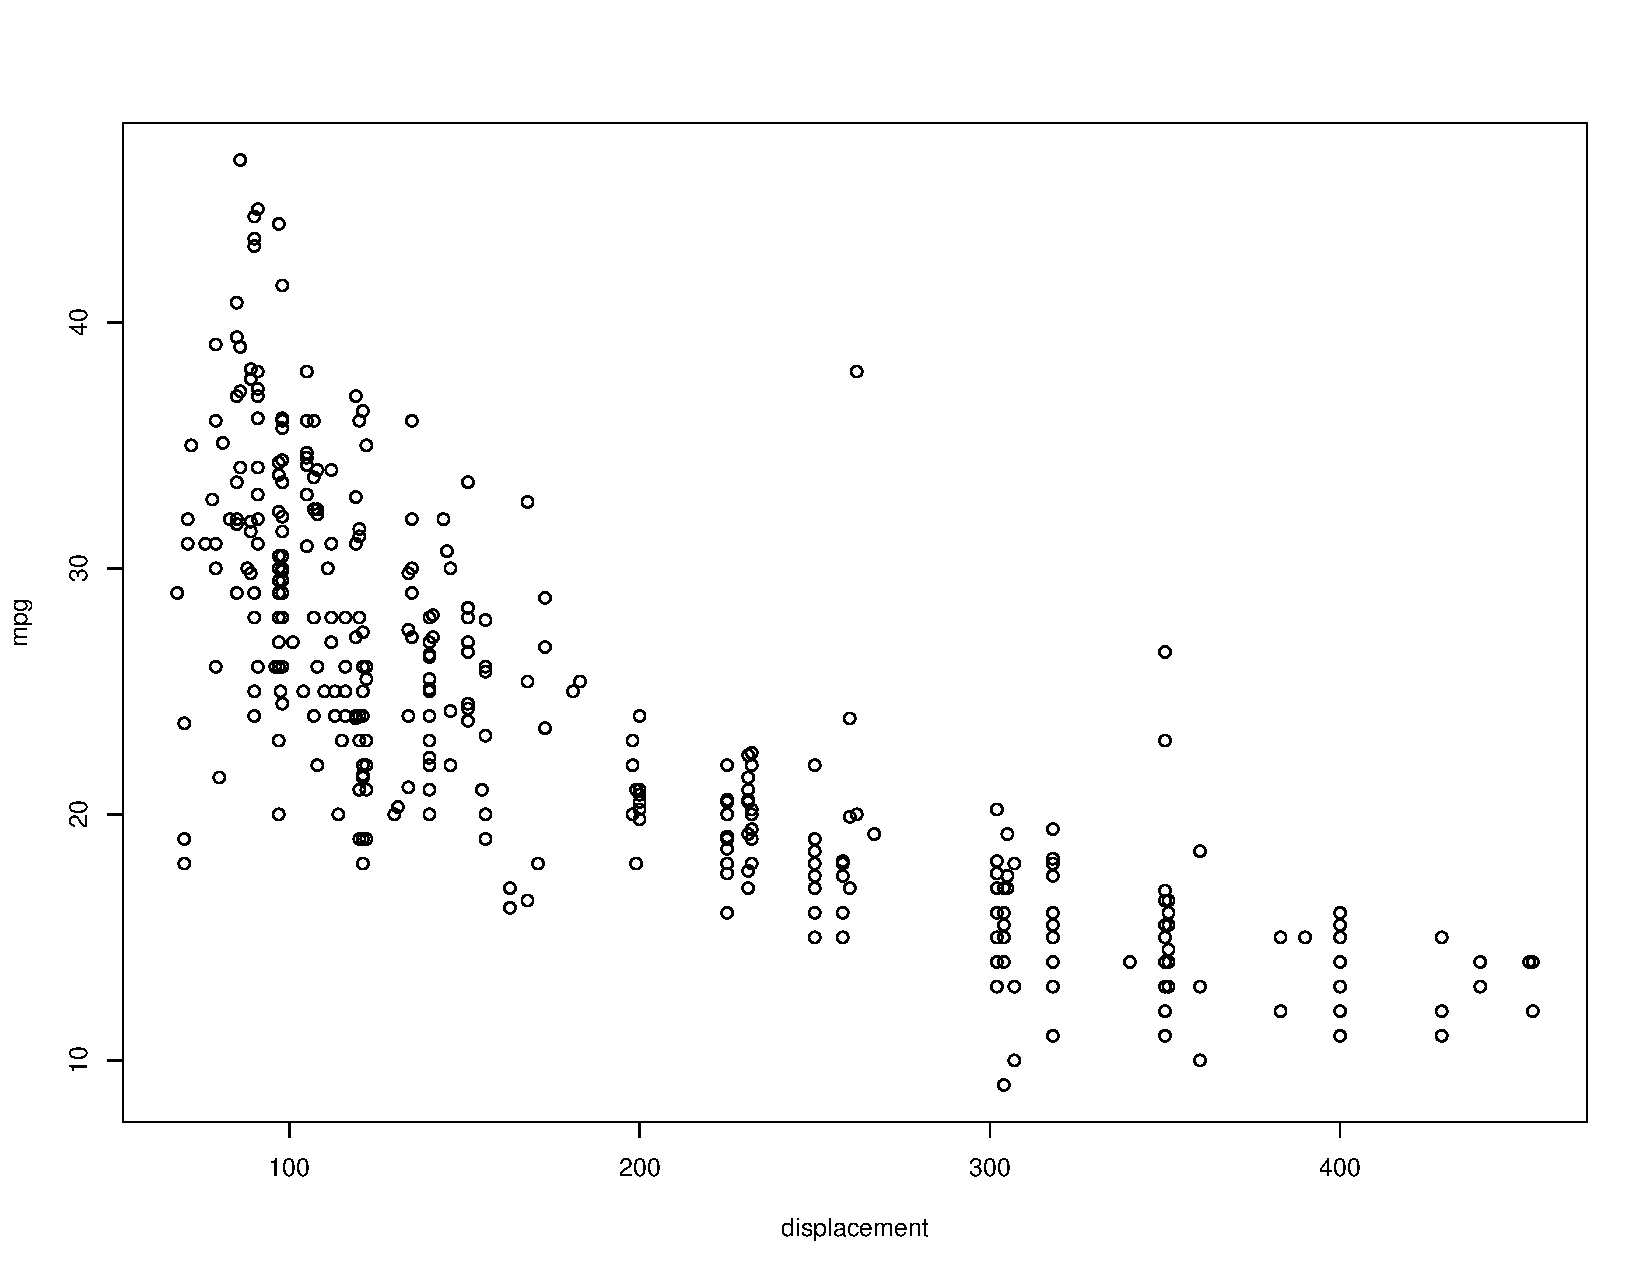
\includegraphics[width=\textwidth]{graphs/scatterDis.pdf}
        \caption{(displacement, mpg)}
        \label{fig:displacement}
    \end{subfigure}
    \begin{subfigure}[b]{0.3\textwidth}
        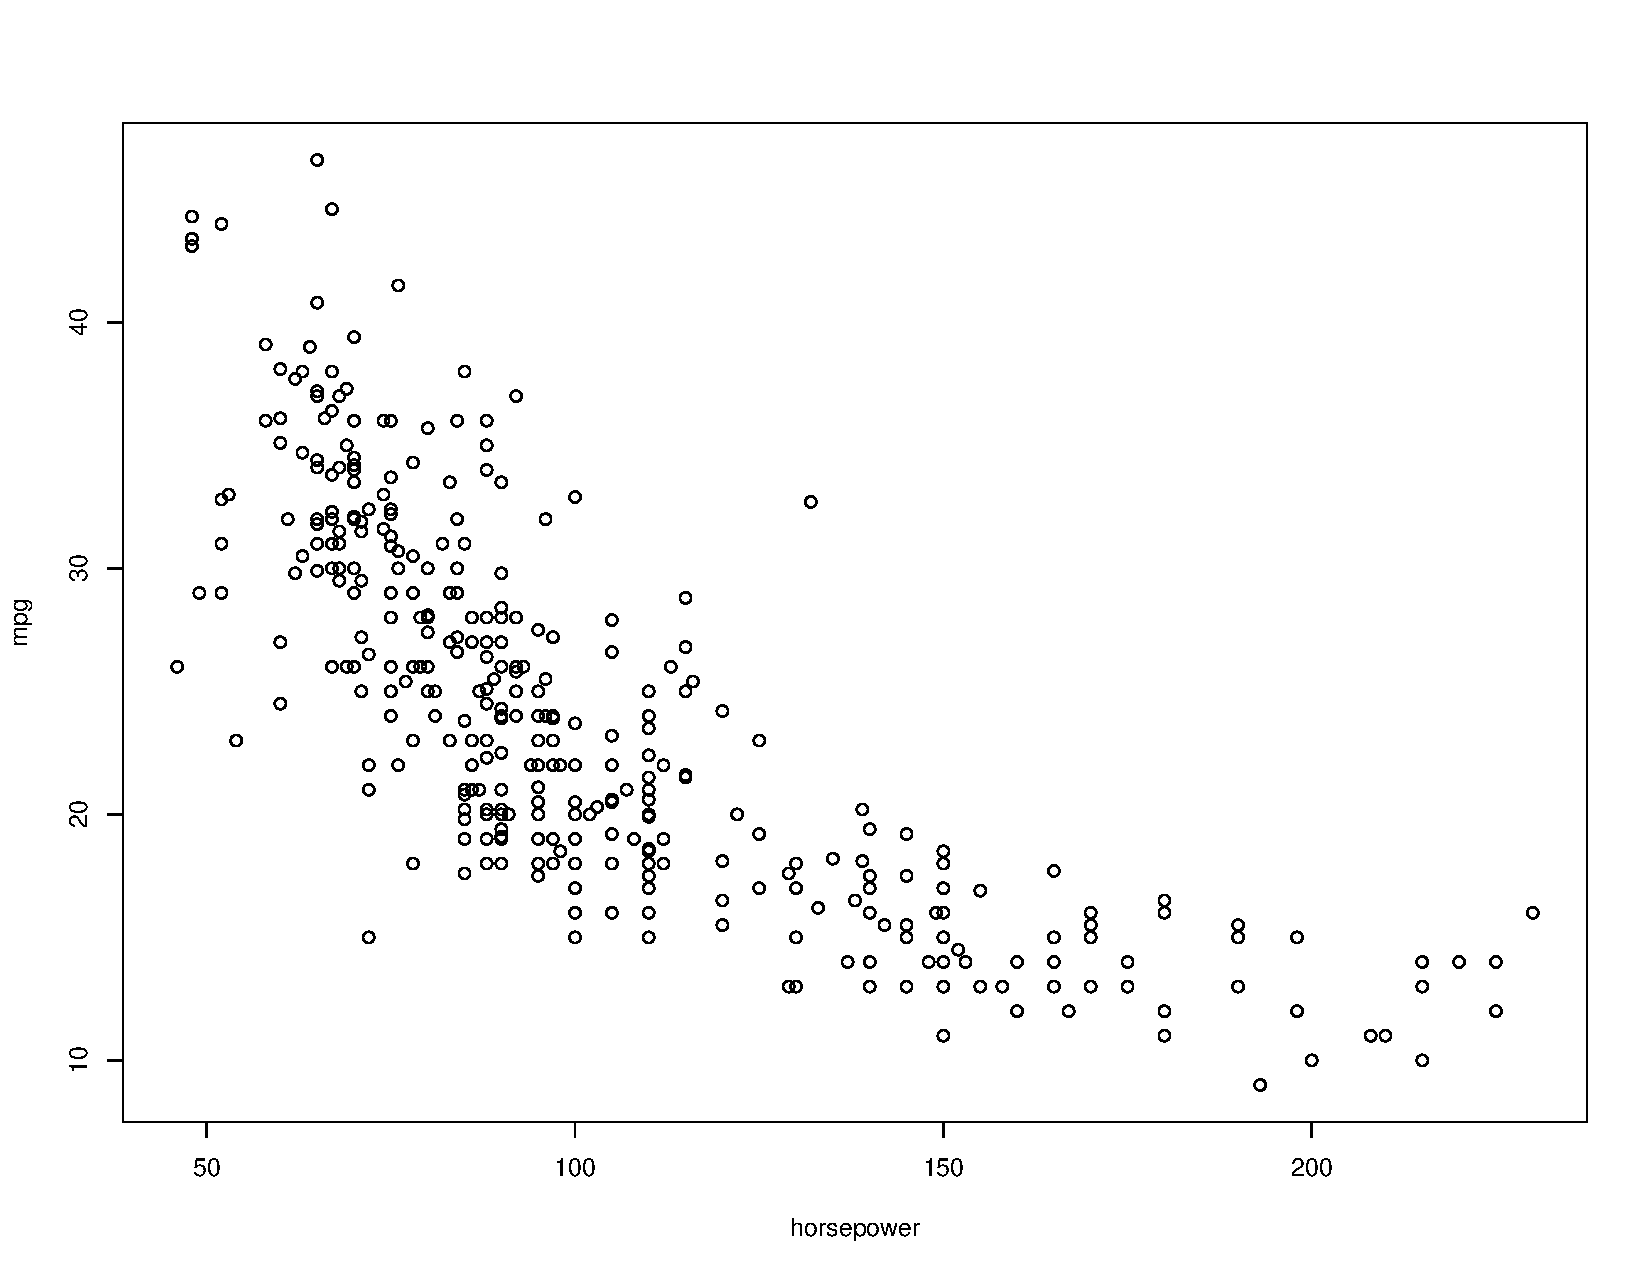
\includegraphics[width=\textwidth]{graphs/scatterHor.pdf}
        \caption{(horsepower, mpg)}
        \label{fig:HP}
    \end{subfigure}
    \begin{subfigure}[b]{0.3\textwidth}
        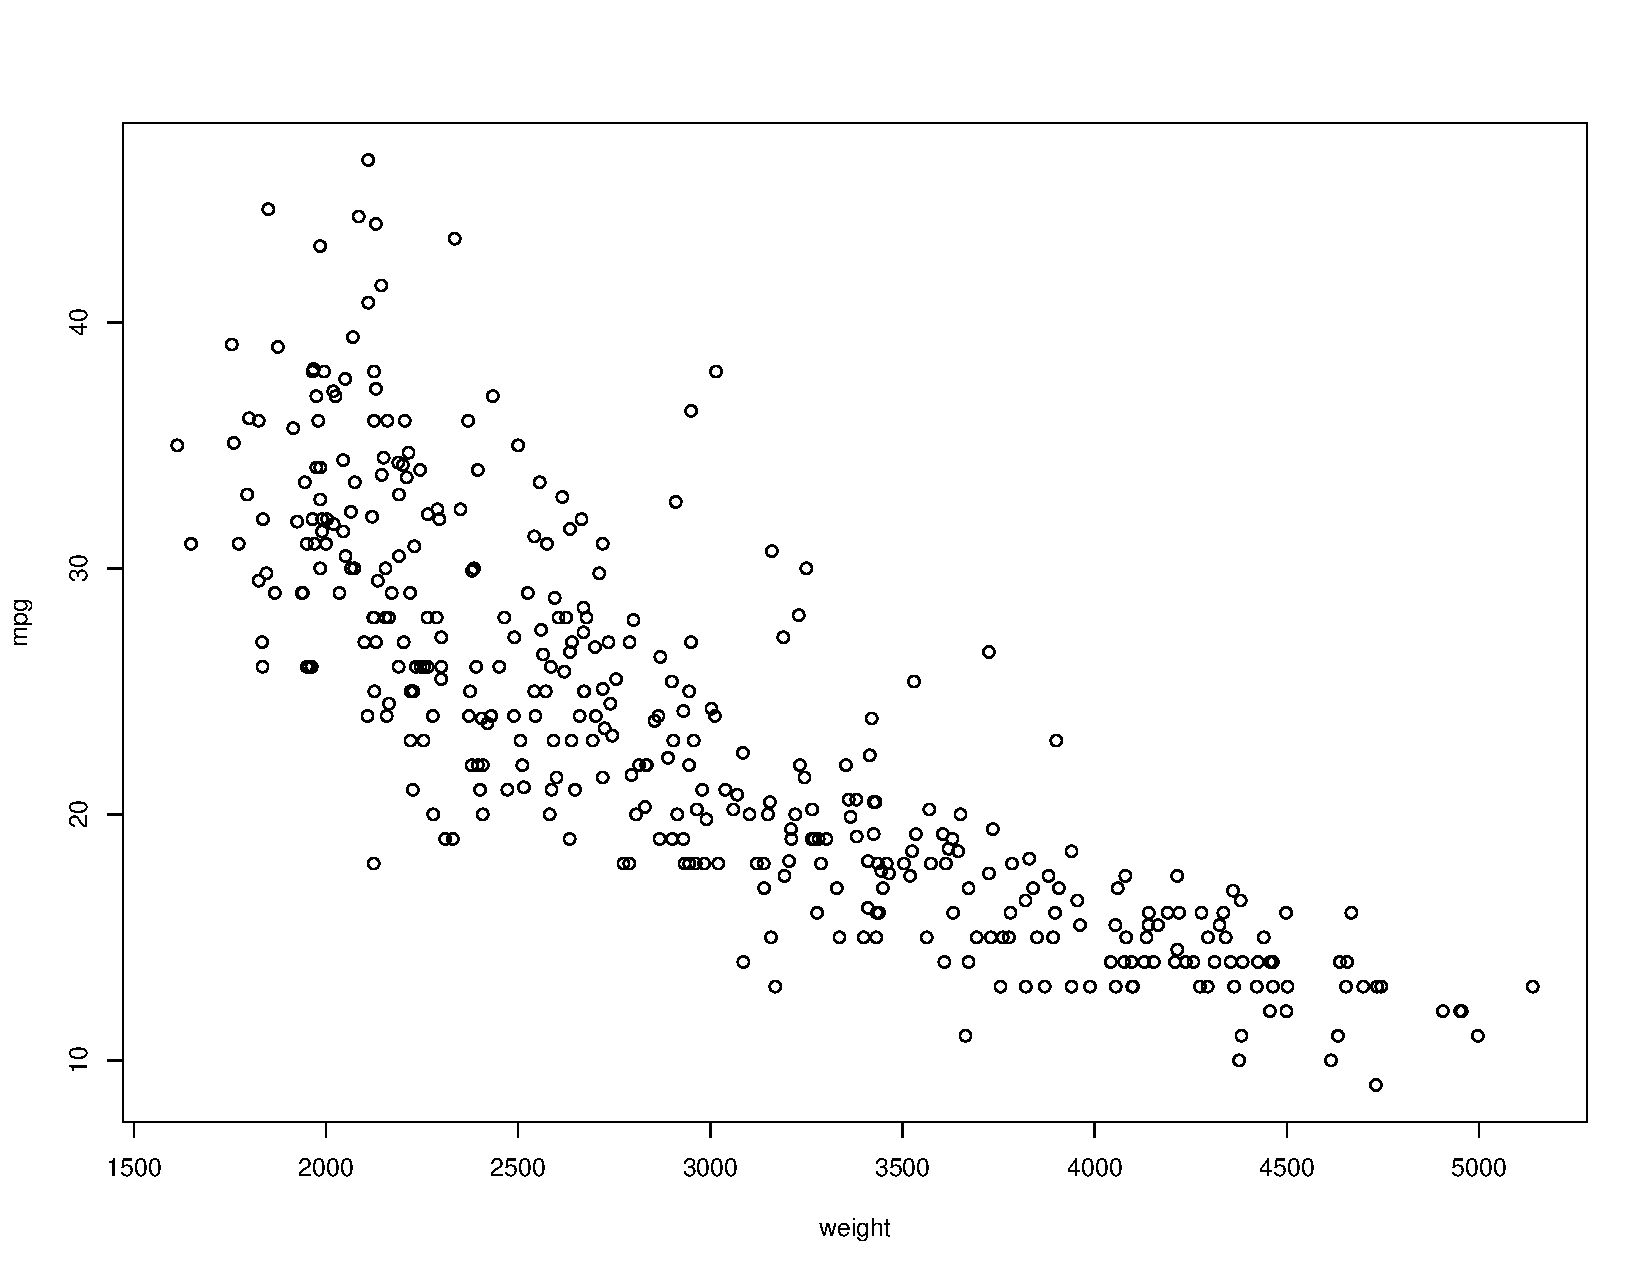
\includegraphics[width=\textwidth]{graphs/scatterWei.pdf}
        \caption{(weight, mpg)}
        \label{fig:HP}
    \end{subfigure}
    \begin{subfigure}[b]{0.3\textwidth}
        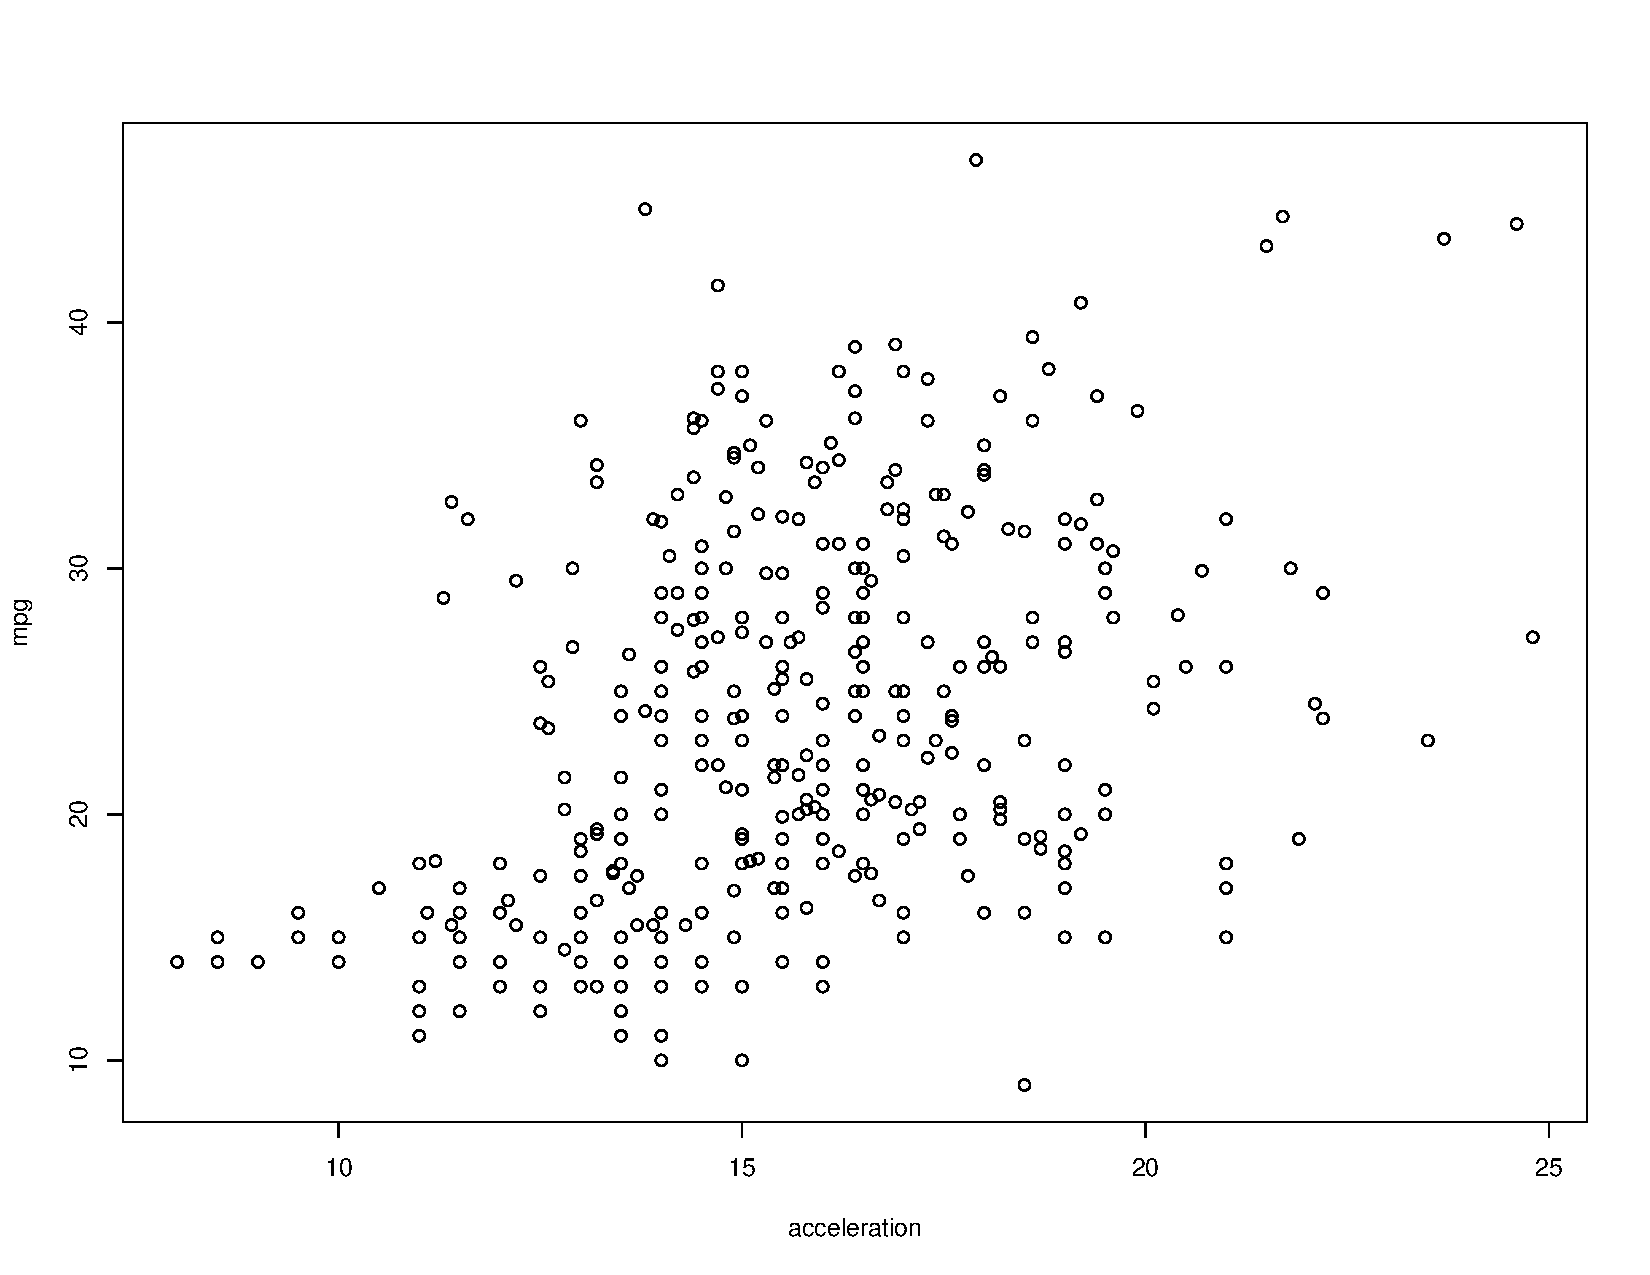
\includegraphics[width=\textwidth]{graphs/scatterAccel.pdf}
        \caption{(acceleration, mpg)}
        \label{fig:HP}
    \end{subfigure}
    \begin{subfigure}[b]{0.3\textwidth}
        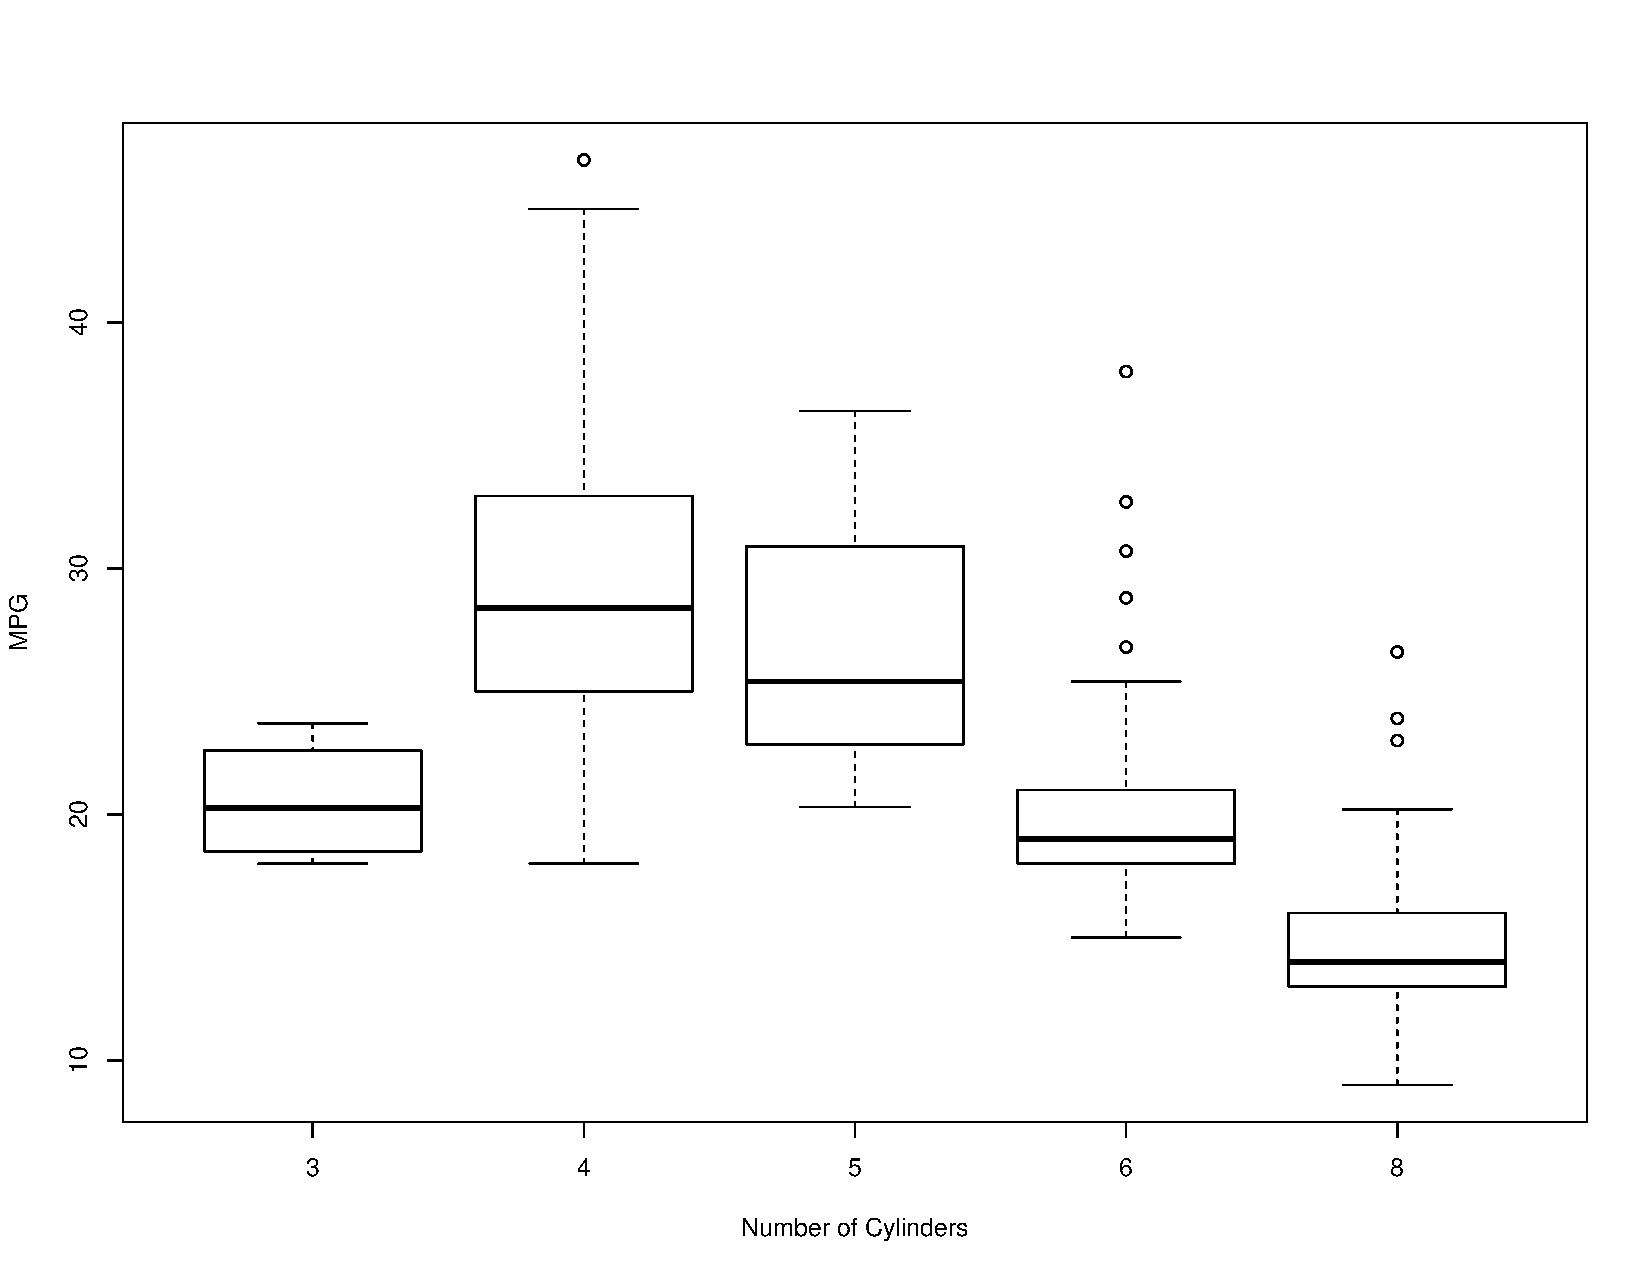
\includegraphics[width=\textwidth]{graphs/boxCyl.pdf}
        \caption{(cylinders, mpg)}
        \label{fig:HP}
    \end{subfigure}
\caption{Plots of Features and Miles per Gallon}
\end{figure}

%Question 4
\question
The scatterplot between cylinders and mpg (figure a) is not easy to interpret, so we converted it to a boxplot (figure f) and found that, though cylinders and mpg appear to be negatively related (that is, a higher number of cylinders typically corresponds to lower mpg), there is much variation within each class. The relationship between displacement and mpg is more obvious, as the scatterplot shows a strong, negative relationship between the two. As displacement increases, mpg decreases. Similarly, horsepower and weight both have clearly negative relationships with mpg. Lastly, acceleration and mpg appear to have no discernible relationship, so acceleration will likely not be a good predictor for mpg.

%Question 5
\question
\begin{rc}
           Cyl      Displ         HP     Weight     Accel
mpg -0.7776175 -0.8051269 -0.7784268 -0.8322442 0.4233285
\end{rc}
The above is a table of correlation coefficients for each feature and mpg. Since they each have correlation coefficients with an absolute value above 0.75, it appears that Cyl, Displ, HP, and Weight will have important, negative effects on mpg. The value of the Accel correlation coefficient is weak, at 0.42, so we do not expect it to impact mpg.

%Question 6
\question
\begin{rc}
              cylinders displacement horsepower     weight acceleration
cylinders     1.0000000    0.9508233  0.8429834  0.8975273   -0.5046834
displacement  0.9508233    1.0000000  0.8972570  0.9329944   -0.5438005
horsepower    0.8429834    0.8972570  1.0000000  0.8645377   -0.6891955
weight        0.8975273    0.9329944  0.8645377  1.0000000   -0.4168392
acceleration -0.5046834   -0.5438005 -0.6891955 -0.4168392    1.0000000
\end{rc}
Above is a correlation matrix for the features. The features appear to be strongly, positively correlated with each other. For instance, a higher number of cylinders is associated with greater displacement, more horsepower, and a heavier car. The only exception to this is the acceleration feature, as it has relatively weak, negative correlations with the other features.

%Question 7
\question
\begin{figure}
\centering
    \begin{subfigure}[b]{0.7\textwidth}
        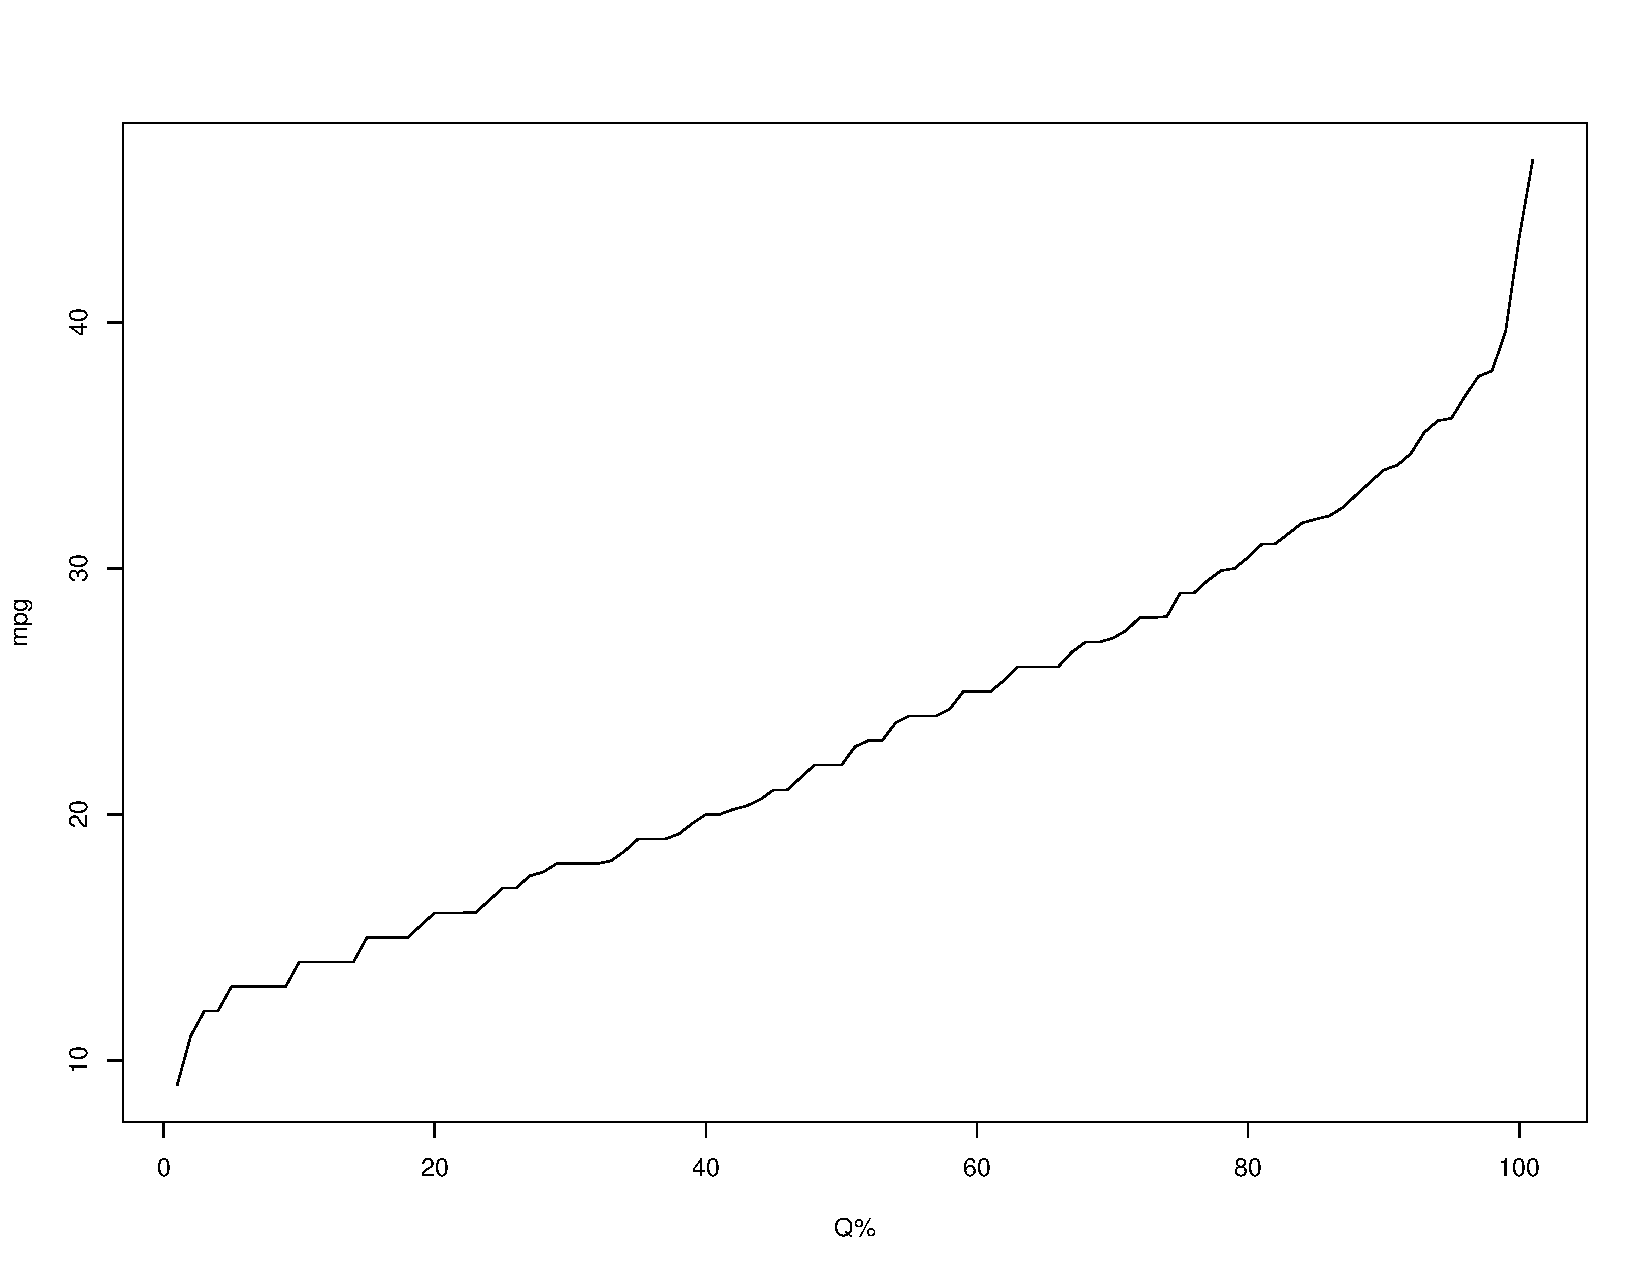
\includegraphics[width=\textwidth]{graphs/qmpg.pdf}
        \caption{(Increasing Quantile Plot for MPG}
        \label{fig:quantile}
    \end{subfigure}
\caption{Increasing Quantile Plot for MPG}
\end{figure}

The above is an increasing quantile plot for the target variable, mpg. It can be interpreted by following the x-axis for a percentage of interest and checking the corresponding mpg value. For example, the 40th percentile of cars in the data set averages 20 miles per gallon. The curve increases at a relatively consistent rate until the mid-90th percentile, when it increases steeply. This is due to some outlier vehicles that get exceptionally high gas mileage.

%Question 8
\question
Our method for splitting the cases into lower and upper thirds was as follows: first, we assigned a variable, p, to function as percentage. Then, we fed that into the quantile function, where mpg was the discriminator. This split the n=392 cases into quantiles, where the (approximately) four cars with the lowest mpg in the data set were assigned the first percent, and the (approx) four cars with the highest mpg were assigned the hundredth percent. So, the lower third of mpg cases, LOWmpg, were those spanning the 0th percentile to the 34th, and the upper third of mpg cases, HIGHmpg, were those running from the 67th percentile to the 100th. The R code which demonstrates this is below:
\begin{rc}
> p <- seq(0, 1, 0.01)
> q <- quantile(mpg, probs=p)
> lowq <- q[0:34]
> highq <- q[67:101]
> LOWmpg <- Auto[mpg <= max(lowq),]
> HIGHmpg <- Auto[mpg > min(highq),]
\end{rc}

%Question 9
\question
DISPLAY MORE HISTOGRAMS

%Question 10
\question
Cylinders: The Low vs High mpg histograms for the cylinders feature shows that the overwhelming majority of cars with high mpg have four cylinders, while most of the cars with low mpg have six or eight cylinders. Cylinders appears to be a feature with strong predictive power.

Displacement: The histograms indicate that the cars with low displacement typically have higher mpg, while cars with higher displacement typically have lower mpg, though there are outliers on both histograms. This likely means that a lower displacement value could lead to a higher mpg.

Horsepower: The high mpg cars typically have horsepower values that are distributed at lower levels, while low mpg cars have horsepower values that are approximately normally distributed, though centered at higher levels of horsepower. While it appears that cars with a higher horsepower have lower mpg, the data is spread widely enough that further investigation of this feature is warranted.

Weight: High mpg cars typically weigh fewer pounds that low mpg cars, with the former's distribution being slightly right-skew, and the latter's slightly left-skew. We could discriminate between high and low mpg cars by saying that cars weighing above 3000 would likely have low mpg, while lighter cars would have high mpg, but the histogram alone does not provide a definitive answer.

Acceleration: Acceleration, for both high and low mpg, is the feature that is closest to having a normal distribution. These histograms do not show a clear difference in the values of acceleration for high mpg and low mpg cars. This feature would be the least indicative of whether a vehicle has low or high mpg.

From the histograms, cylinders and displacement appear to be the features with the most discriminitory power.

%Question 11
\question
For LOW mpg:
\begin{rc}
            Cyl     Displ        HP    Weight     Accel
Mean   7.407692 315.30769 145.62308 3937.3308 13.778462
StdDev 1.009230  71.11404  35.84101  557.1857  2.649294
\end{rc}
For HIGH mpg:
\begin{rc}
             Cyl     Displ       HP    Weight     Accel
Mean   4.0833333 106.40152 74.39394 2226.0909 16.560606
StdDev 0.3915455  26.42225 13.88434  345.8779  2.519989
\end{rc}

%Question 12
\question
\begin{rc}
   cylinders displacement   horsepower       weight acceleration 
   35.148517    31.517470    21.210516    29.865390     8.708918 
\end{rc}
The above table is the discriminating ratio for each of the five features. Cylinders has the most discriminatory power at a score of 35.15, while acceleration has the least discriminatory power at 8.71. It appears that displacement and weight also have good discriminatory power with scores around 30, while horsepower may be a good indicator as well.

%Question 13
\question
TO BE COMPLETED

%Question 14
\question
The previously defined classes, LOWmpg and HIGHmpg, will be used as our training set, while the cases falling in between the 33\% and 66\% quantile, which have not been explored yet, will be used as the test set. 

The automatic classifier will follow a simple rule using the sum of the feature scores (fscore) for each case and a chosen value A. A case is considered to have low mpg if its score is less than A and high mpg otherwise. 

Starting with A=1, we apply the classifier to our training set to get the following results:
\begin{rc}
         predLow     predHigh
trueLow  0.99230769 0.007692308
trueHigh 0.03030303 0.969696970
\end{rc}
Looking at this confusion matrix, we can see that when A=1, the classifier has a high accuracy when applied to the training set. Of the 130 total lowMPG cases, it was able to properly identify 129, and it only incorrectly labeled 4 of the 132 highMPG cases. 

For the test set, we first define its true class by classifying any cases with mpg higher than median of all mpg values as high mpg and low mpg otherwise. Notice that the training set already follows this rule since LOWmpg is a subset of the lower 50\% quantile, consisting of 33\% and below, and HIGHmpg is a subset of all cases above the 50\% quantile (above 66\%). Applying the classifier with A=1 to our test set gives the following confusion matrix:

\begin{rc}
         predLow    predHigh
trueLow  0.6666667 0.3333333
trueHigh 0.1406250 0.8593750
\end{rc}

When applied to the test set, there is a noticeable drop in accuracy. It was able to correctly label 55 of the 64 high mpg cases and only 44 of the 66 low mpg cases. 

\begin{rc}
> Ctrain2
           predLow   predHigh
trueLow  0.99230769 0.007692308
trueHigh 0.07575758 0.924242424

> Ctest2
           predLow  predHigh
trueLow  0.7575758 0.2424242
trueHigh 0.3281250 0.6718750
\end{rc}

When A=2, the classifier's accuracy decreased for the training set and gave mixed results for the test set. For the training set, the low mpg numbers are the same as they were previously. However, the classifier did a worse job identifying high mpg cases. Now, there are 10 incorrect rather than 4, which is about a 4.5\% decrease in accuracy compared to when A=1. 

For the test set, At A=2, the classifier does a better job identifying the low mpg cases but a worse job for the high mpg cases. It accurately classified 6 more low mpg cases than previously, about a 9.1\% boost in accuracy. However, it now makes an additional 12 incorrect classification for high mpg cases, which is about a 18.75\% loss in accuracy from when A=1.

The list of full scores for both sets only contain odd values (ranging from -5 to 5), so any even value A would have the same results as when A=A+1. Therefore, the results for A=0 is the same as for A=1, and A=3 is the same as A=2.

The differences between the results for the training set and the test set suggest that this automatic classifier could use some improvement. The threshold levels for the classifier function, which were determined from the standard deviations found in the training set, appear to serve very well in classifying the training set at any value of A but are much less adequate for the test set. Optimizing the A value is not enough to make this automatic classifier effective. We may need to revise the calculation for discr(F). 

%determine which A is best?
%suggestions on improving the classifier?
\end{document}
